\documentclass[12pt]{article}
\usepackage[ampersand]{easylist}
\usepackage{amsmath}
\usepackage{amsfonts}
\usepackage{amssymb}
\usepackage[obeyspaces]{url}
\usepackage{hyperref}
\usepackage{graphicx}

\title{Monitoring Memory and CPU Usage for Processes in Linux}
\author{Jatczak, David \and McNabb, Trent}

\begin{document}
	
	\maketitle
	
	\section{Introduction}
	
	\subsection{Context}
	Addressing this issue requires knowledge of what information is relevant to the calculation of memory and CPU (Central Processing Unit) resources, and how to get that information. Specifically, knowledge of the Linux \path{/proc/} files is needed.
	
	\subsection{Problem Statement}
	Computer users who are used to Windows might use \emph{Ctrl+Alt+Delete} when they wish to see which processes are running and how much of the system's resources those processes are consuming. They may not be comfortable using the terminal to run commands that would display that information, and they might prefer to see the information in a GUI (Graphical User Interface). A program that is accessible via the \emph{Ctrl+Alt+Delete} keyboard shortcut that resembles the Windows Task Manager is needed. It should allow for a clear and easy view of which processes are running and what resources each process is using. It should be easy to terminate a running process.
	
	\subsection{Result}
We have created a program that is called on our system using the \emph{Ctrl+Alt+Delete} keyboard shortcut. The program uses a GUI to display the running processes and the percentage of CPU resources and memory used by each process. The program allows users to easily select and terminate processes.
	
	\subsection{Outline}
	The rest of this report is structured as follows: Section 2 presents background information, including information about calculating system resource usage by specific processes using the Linux \path{/proc/} file; Section 3 describes in detail the program that we have written, which is the result of this project; Section 4 evaluates the result of the project, primarily through a usability study; Section 5 is the conclusion.
	
	\section{Background Information}
	The Linux \path{/proc} file system stores information about processes and also other system information.
Each process has a directory in the \path{/proc/} directory\cite[p. 792]{text}.
The directory is created at \path{/proc/[PID]/}, where PID (Process Identifier) is the process identification number. Each of these directories include a 'stat' file, a 'statm' file, and a '/status' file. In addition to the information about each process, there is also system information, i.e. the \path{/proc/cpuinfo} file and the \path{/proc/meminfo} file.\\
	The Resident Set Size in the number of pages that the system currently has in real memory.
	If we multiply that by the page size, that gives the amount of RAM (Random-access Memory) currently used by the process.
	If we divide that by the total amount of memory used by the system, that will give us the percentage of system memory used by the process.
	The calculation is:\\
	
	$$ \frac{\text{Resident Set Size} \times \text{Page Size}}{\text{Total System Memory}} $$
	
	Information about the resident set size of a process can be found is \path{/proc/status/statm} \cite{manProc}.
	Information about the total system memory can be found in \path{/proc/meminfo} \cite{manProc}.\\

A CPU can either be running or idle.
If it is running, it can be running a user space program, or running the kernel \cite{scoutBlog}.
If you add the time it is running the kernel, plus the time it is running a user space program, plus the amount of time it is idle, you get what we will call the Total CPU availability.
The percentage of CPU usage by a process is the amount of time that the CPU is running that specific process, divided by the Total CPU availability multiplied by 100.
The percentage of total CPU usage is the amount of usage, divided the total CPU amount, multiplied by 100, where the amount of usage is the time running user space programs plus the time running kernel space programs.\\
The amount of time that a process has been running in user mode can be found in \path{/proc/PID/stat}. \cite{manProc}
The total time spent by the CPU running user space processeses and the amount of time running the kernel can be found in \path{/proc/stat} \cite{manProc}.\\
	
	
Shortcuts, also known as hotkeys, that give functionality to applications are typically handled by an event handler.
Whenever a user presses a key on an operating system, an event is made and sent out for the event handlers to handle.
There are many more types of events than key presses and key releases, such as mouse movements, and GUI events.
Event handlers are in event loops. Event loops are embedded in applications themselves and/or in the operating system. Simple processes such as shell tools do not typically have event handlers, but many modern applications do. The typical structure of an event loop is that goes through the queue of events it has, does what it needs and then chooses to dispatch the event or not, afterwards waiting for more events. 

The Qt framework offers a library that gives GUI functionality and is based in C++, but it also used in other languages such as Python where it has been ported.
The Qt framework has an event loop and receives its events from windowing systems such as X11 or Wayland.
If you are interested in this topic, it is explained further by Thiago Macieira in his powerpoint on the Qt event loop\cite{QtSlides}.

For this text, we use X11 as our window system.
X11 is the base of the GUI system for Linux.
It handles all the communication between the user input and other windows because it is the framework that other applications are working off.
X11 has its own event loop, and is basically at the top of the hierarchy of event loops.

To interact with X11's event loop, you require a library such as Xlib or XCB.
XLib was made by the same company that created X11.
XCB is a faster alternative to Xlib and is asynchronous.
Both of these libraries communicate with X11 via binary because X11 uses a client-server design for its system.

Unity is the desktop environment for Ubuntu, it operates with X11 (by default). Unity is able to use .desktop files to launch applications.
These .desktop files are in plaintext and assign key-value pairs such as what command to execute.
An option to launch the files upon startup is done by putting them in \path{~/.config/autostart}.
Unity also has custom shortcuts available that can execute commands.
The configuration of shortcuts are separate for each each user and are located in the user's /path{~/.config/dconf}.
The configuration files are not plaintext, so the only way to change the configurations by terminal is through the command 'gsettings'.


	
\section{Result}

The GUI layout was created in Qt Designer, which outputs a '.ui' file, which is an file in XML (Extensible Markup Language).
That '.ui' file is compiled by PyQt5 into the files that run the GUI.
For our program, those files were 'mainwindow.cpp', 'mainwindow.h', and 'mainwindow.cpp', and the python class that allows our program, 'Overseer.py', to interface with the gui, 'UImainwindow.py'.
'Uimainwindow.py' has a class called Ui\_MainWindow that allows the creation of Ui\_MainWindow objects.
These files are all generated by the PyQt5 compiler, and any changes in them are made by changing and recompiling the '.ui' file.
When the main function is run in 'Overseer.py', it creates an Ui\_MainWindow object, runs the OverseerMainWindow function and tells the Ui\_MainWindow object to show on the screen.\\
The OverseerMainWindow function creates the the model for the table that holds the data so that the UI can display it.
It creates an instance of the Proc class from 'proc.py'.
The OverseerMainWindow function calls the udpate function, which updates the data by calling the readData function on the Proc object and then updates the view by calling the updateView function.
It repeats this once every second.\\
The Proc object stores the following data: a dictionary called processList, a UserList object called userList, from 'userlist.py', an integer called totalMem, and two lists called cpu and openWindows.\\
The readData function runs the functions that populate each of those data members.
readTotalMem gets the total memory usage from \path{/proc/meminfo}.
See Figure ~\ref{figTotalMem}.
The circled data is the data stored as totalMem and the freeMem in the Proc object.
\begin{figure}[h]
	\centering
	\textbf{Total Memory}\par\medskip
	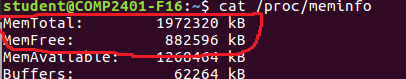
\includegraphics{totalMem}
	\caption{Output of \url{cat /proc/meminfo}}
	\label{figTotalMem}
\end{figure}

readCupTimes gets the CPU infomation from '/proc/stat'.
See Figure ~\ref{figCPUInfo}.
The circled data are the numbers put in the list cpu.
The circled data are the numbers put in the list cpu.
This in the combined data for all processors in the system.
The first number is the time spent in user mode, and it is stored in cpu[0]
The third number is the time spent in system mode, and it is stored in cpu[3]
The fourth number is the time spent in idle, and it is stored in cpu[4].
None of the other numbers are relevant.
\begin{figure}[h]
	\centering
	\textbf{CPU Information}\par\medskip
	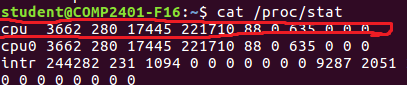
\includegraphics{totalCPU}
	\caption{Output of \url{cat /proc/stat}}
	\label{figCPUInfo}
\end{figure}

Overseer is able to calculate its CPU usage and RAM usage through polling.
The interval for polling is every second.
The data that is used for polling is describing running processes and the operating system and is stored on \path{/proc}.
Reading these files may seem like a strain, but there should not be any overhead from IO blocking since these files in \path{/proc} are virtual files and not actual files on a disk.
Virtual files are stored only on RAM (Random-access Memory), also known as the main memory.
In theory you should be able to read all the info from \path{/proc} almost instantly.
Thus having 1 second of polling should not be too bad for a single threaded program.

When all this data is collected from \path{/proc}, we also perform our CPU and RAM usage calculations as well as collecting a list of users.
The list of users is collected at the start of the poll cycle.
Collecting a list of users gives overhead as there is possible IO blocking from reading \path{/etc/passwd} because this is not a virtual file but an actual file on the disk.
Information on open windows in the window manager is collected through \path{wmctrl} and might give overhead as well depending on how wmctrl operates; window information is also collected in each poll cycle.

The original goal was to have Overseer launch upon startup and it would sit in the system tray, where it would show the window when the shortcuts \emph{Ctrl+Alt+Delete} or \emph{Ctrl+Shift+Escape} was pressed.
Overseer would have used an event handler for detecting the shortcuts (key press events).
If a key release event was detected for either key in a shortcut before all 3 keys having a key press event, the check for the shortcut would fail.
Implementation for putting a .desktop file in \path{~/.conf/autostart} did manage to get the program to launch on startup. But if the user were to log out and log back in, it would not launch again.

However, the main crux is the issue of reading events from X11 within the main thread of the application, which Qt operated off.
The Qt framework only provided ways to have working shortcuts if the Qt application itself is in focus, meaning it is unable to read key presses when the Qt application is minimized or selected to receive user input.
So another library was needed to read key press events, which led to Xlib.

Utilizing Xlib to read key presses with Python 3.5.2 is possible.
There is an example at \path{/usr/share/doc/python3-xlib/examples/record_demo.py} that illustrates reading events.
However, due to our lack of knowledge with Xlib and the poor documentation \cite{badDocumentation} for the Python version of Xlib, the event loop could not be changed to our liking.

Essentially the call back loop handles all the events coming from X11, then keeps calling itself to handle more events.
This call back loop was not possible to implement in our application's main thread because Qt operates off the main thread.
For example if \emph{time.sleep(5)} were to be executed in the main thread, the GUI would stop working all together and look frozen for 5 seconds.
This call back loop was the only thing executing so Qt did not operate.

It was thought it would be possible to implement the Xlib call back loop in another thread, a QThread, where this 2nd thread would check for key press events with its callback loop while the main Qt GUI thread would run.
However, it is incredibly dangerous when Xlib is used out of the main thread, as was explained to us by the Qt Core Maintainer Thiago Macieira over IRC.
Also to add, multithreading is not a wise idea with Qt in general.
The reason is you could have more overhead to Qt's main event loop if your threads were sending more events to the main thread's event loop. This is explained further by Qt's web page\cite{QtThreading}.

Thus XCB was turned to instead, as another way to read events.
A derived class of QAbstractNativeEventFilter, a class in the Qt framework, was created to handle the events coming from X11.
The type \url{xcb_generic_event_t} is sent to \url{QAbstractNativeEventFilter} by Qt.
Unfortunately, Python 3.5.2 does not recognize that type of data, and the PyQt5 library does not have an implementation of this data type either.
An XCB library was needed to understand the \url{xcb_generic_event_t} data.

Due to our entire application being programmed in Python 3.5.2, there are no decent libraries of XBC available.
Most libraries for XBC on Python are in the 2.x version of Python, e.g. \url{https://xcb.freedesktop.org/XcbPythonBinding/}.
Search engine results led to other XBC implementations in Pythyon 3.x such as \url{https://github.com/samurai-x/samurai-x/tree/master/pyxcb/pyxcb} or \url{https://github.com/tych0/xcffib}.
Both were unsuccessful for deciphering key press events from \url{xcb_generic_event_t} data.
There was some progress in deciphering the data, but there are many missing functions and constant values such as \url{XBC_MOUSE_PRESS}. The work can be seen from \url{http://github.com/Davidj361/Comp3000Group5/tree/global-shortcuts} and \url{http://github.com/Davidj361/Comp3000Group5/tree/global-shortcuts-method2}

Finally shortcut functionality was achieved with Unity's custom shortcuts.
Our Overseer does not deal with any events in the code, it merely interacts with Unity's custom shortcuts system.
Our application does not launch no longer on startup with a .desktop file, but instead launches from a bash file when a shortcut is pressed which in turn opens our Overseer application.
\emph{Ctrl+Alt+Delete} or \emph{Ctrl+Shift+Escape}
Unfortunately the \emph{Ctrl+Shift+Escape} does not work.
The reason is because Ubuntu's shortcut manager does not work with \emph{Escape} as part of a shortcut, as illustrated in this bug report \url{https://bugs.launchpad.net/ubuntu/+source/compiz/+bug/158855}.

The applications tab in Overseer utilizes \path{wmctrl}, a 3rd party tool, to interact with windows in the desktop environment.
It collects information on windows showing in desktop environment and also gives the functionality for switching to a window.
Unfortunately \path{wmctrl} also collects information on junk windows such as 'Hud', 'unity-dash', 'unity-panel', 'unity-launcher', and 'XdndCollectionWindowImp', even if it's not on the desktop environment's taskbar.

Selections on the \emph{QtTableView}s in the process tab and applications tab has issues because Python does not have pointers.
It is hard to utilize Model View Controller design, which is the basis of \emph{QtTableView}, because we cannot link our data straight from Overseer's Proc class as a model to a QtTableView.
Instead, there's a poll cycle and new data is grabbed, all of the entries in each \emph{QtTableView} is erased and reinserted.
However, this gets rid of our selection every poll cycle. 
So Overseer remembers a \emph{PID} if there was a selection before the erase and reselects by iterating over the entire list in the \emph{QtTableView} looking for a matching PID, otherwise leaves no selection if not found.
Sadly this adds overhead to the main thread.	
	
	\section{Evaluation}
	Evaluation goes here.
	
	\section{Conclusion}
	
	\subsection{Summary}
	Summary and highlights.
	
	\subsection{Relevance}
	Relevance with respect to the course topic.
	
	\subsection{Future Work}
	Question for TA -- future work in the field of this project, or ways that the project application itself could be continued on.
	
	
	\setcounter{secnumdepth}{0}
	\section{Contributions of Team Members}

\ListProperties(Hide=100, Hang=true, Progressive=3ex, Style*=-- ,
Style2*=$\bullet$ ,Style3*=$\circ$ ,Style4*=\tiny$\blacksquare$ )

For reference
\begin{easylist}
& Blah
& Blah
&& Blah
&&& Blah
&& Blah
&&&& Blah
&&&&& Blah
\end{easylist}		
	
\subsection{David Jatczak}
\begin{easylist}
& All of following classes: Process, CPU , UserList, and UserEntry
& For Proc class:
&& Implemented readcpuTimes, readOpenWindow; obtaining: process times, process CPU usage percentage, process paths, their permissions, process state.
& For OverseerMainWindow class:
&& Implemented Right-click context menus, selection logic for QTableViews, button logic, setupgsettings, setupLaunchScript, and setupShortcuts
& For the Project Report Document:
&& For the Background Section:
&&& Explaining Shortcuts, Events\&Event-Handlers\&Event-loops, X11, Unity, .desktop files
&& For the Results Section:
&&& Describing polling, overhead in polling, the failures of utilizing event handling, Unity's shortcut functionality, wmctrl, difficulty with MVC in QTableView, selection logic in QTableView
&& Proof read Trent's text
& Placement of GUI elements
& Reading htop's and top's source code to find RAM \& CPU usage calculations
& Research in event handling
\end{easylist}

\hfill\break
For more detail on contributions: \url{http://github.com/Davidj361/Comp3000Group5}
	
	
	
	\begin{thebibliography}{3}
	\bibitem{QtSlides} Thiago Macieira - Qt Core Maintainer \url{http://github.com/boostcon/cppnow_presentations_2013/blob/master/mon/qt_event_loop.pdf?raw=true}
	\bibitem{manProc} Proc(5) - Linux Manual Page
	\url{http://man7.org/linux/man-pages/man5/proc.5.html}
	\bibitem{text}{Tanenbaum, A. S. (2015). \emph{Modern operating systems.}}
	\bibitem{scoutBlog} Understanding Linux CPU stats \url{http://blog.scoutapp.com/articles/2015/02/24/understanding-linuxs-cpu-stats}
	\bibitem{badDocumentation} \url{/usr/share/doc/python3-xlib/html} \& \url{http://python-xlib.sourceforge.net/doc/html/index.html}
	\bibitem{QtThreading} \url{https://wiki.qt.io/Threads_Events_QObjects}
	\end{thebibliography}{}
	
FIXME: DELETE BELOW

•	Don’t generalize in your introduction, go straight to the point
•	Should be understandable to another student at our level
•	Acronyms should be defined, but don’t use the title, even things like IP. So first time used should be: Internet Protocol (IP)
•	Do not tell a story, do not use future tense, same in past, unless the events must be told in the past.
•	Use simple and short sentences, nothing like 3 lines for 1 sentence
•	1.2 \& 1.3 are related
•	 Number your sections
•	1.1 – what happened before the problem \& your project
•	1.3 – what we have actually achieved
•	1.2 – The motivation, it’s not about us but about the software. Do not put your personal motivations, that can be as an appendix
•	1.4 – To give to the reader an outline, an overview of the upcoming sections so section 2!
•	Section 2, the target audience is the people in our class, people like us.
Section 2
•	Use your own algorithms and on your own examples
•	Careful copy pasting diagrams, not even when cited. But you need to create your own diagrams. Also when copying figures, the original tends to have more elements.
•	When talking about other people’s work (software) don’t be negative and destructive about their work
•	Cite other’s work
•	Only concepts are important, wording is not important, so quotations of people are not needed, put it in your own words.
 
Section 3
•	The core of the work
•	Code is not needed, the design and the logic is what is needed
•	If putting code, should be snippets and short
•	You can use pseudocode, UML diagrams
•	You will make claims. There are 2 types of claims, relevant and irrelevant claims. Also there needs to be evidence! Such as evidence for being fast or easy to use. What is it faster than? What software is it faster than?
•	Be honest, even if it’s not easy for you. Do not hide it.
•	Assume the reader is lazy, explain the contents of figures, i.e. write as if the reader is blind to the figure.
Section 4
•	Evaluation of our work
•	For questionnaires, there’s a pre-quiz to get a background on testers. Also timed the user for doing each task. Final questionnaire is about the application.
•	Use statistical math to support your claims
Conclusion
•	The same thing that’s repeated 3 times


\end{document}
